\section*{Dati e risultati}

L'oscillatore a ponte di Wien si può realizzare seguendo lo schema circuitale riportato in Figura \ref{fig:oscillatore}.
Il circuito è quindi costituito da un amplificatore operazionale UA741 che presenta due due reti di retroazione, una positiva e una negativa.

Analizziamo inizialmente la rete di retroazione positiva e il suo effetto sulla tensione di output $V\ped{out}$.
Questo ramo di retroazione è formato da una resistenza $R$ in serie ad un condensatore $C$, quindi possimo dire che sia un filtro passa alto. Questo primo blocco avrà un'impedenza $Z_4$. L'ingresso non invertente $V^+$ è collegato al comune mediante un parallelo tra una resistenza $R$ ed un condensatore $C$. Questo secocndo blocco avrà un'impdenza $Z_3$.

Quindi grazie al calcolo delle impedenze, analizzando singolarmente la struttura del ramo di retroazione positiva, possiamo trovare la funzione di trasferimento di questo piccolo circuito. Ovvero:
\begin{equation}
	Z_3\,=\,\frac{R}{1 + i \omega C R} \qquad \text{e} \qquad Z_4\,=\,R + \frac{1}{i \omega C}
\end{equation}
quindi otteniamo che:
\begin{equation}
	V\ped{O}\,=\,\frac{Z_3}{Z_3 + Z_4} \cdot V\ped{I}\,=\,\frac{i \omega R C}{(1 + i \omega C R)^2 + i \omega C R} \cdot V\ped{I}
\end{equation}
dove con $V\ped{O}$ abbiamo indicato la tensione in uscita da questo blocco e con $V\ped{I}$ il segnale in ingresso allo stesso.
Quindi, analizzando la funzione appena trovato ci si può rendere conto che rappresenta un filtro passa banda. Inoltre possiamo calcolare il guadagno $\beta$ della retroazione positiva:
\begin{equation}
	\beta\,=\,\frac{V\ped{O}}{V\ped{I}}\,=\,\frac{i \omega R C}{1 - (\omega C R)^2 + 3 i \omega R C}
\end{equation}
Grazie a questa relazione possiamo osservare che se la frequenza del segnale in ingresso $f$ è uguale alla frequenza di risonanza $f_0$ del circuito abbiamo che il segnale in uscita $V\ped{O}\,=\,\frac{1}{3} \cdot V\ped{I}$. Infatti la frequenza di risonanza del nostro filtro passa banda vale:
\begin{equation}
	f_0\,=\, \frac{1}{2 \pi R C} \qquad \text{con} \qquad \omega_0\,=\,\frac{1}{RC}
\end{equation}
quindi se $\omega \,=\, \omega_0$ abbiamo che:
\begin{equation}
	V\ped{O}\,=\,\frac{1}{3} \cdot V\ped{I}
\end{equation}

Quindi grazie a questo noi sappiamo che al'ingresso non invertente $V^+$ dell'amplificatore operazionale abbiamo una tensione che vale un terzo della tensione in uscita dall'amplificatore $V\ped{out}$.
Da questo risultato segue che per ottenere oscillazioni stabili nel tempo anche la tensione all'ingresso inverente $V^-$ dell'amplificatore deve valere un terzo della tensione di output.

Quindi, come nel caso precedente, se analizziamo separatamente questa parte di circuito, ovvero il ramo di retroazione negativo otteniamo che:
\begin{equation}
	A\,=\,1 + \frac{R_v}{R_1} \qquad \text{inoltre} \qquad V\ped{out}\,=\,AV^- \qquad \text{da cui} \qquad V^+\,=\,\frac{V\ped{out}}{A}
\end{equation}
pertanto visto che vogliamo che $V^+\,=\,\frac{1}{3} \cdot V\ped{out}$ si ottiene che $A\,=\,3$ e quindi:
\begin{equation}
	R_v\,=\,2R1
\end{equation}

Quindi fino ad ora abbiamo analizzato i due rami di retroazione dell'oscillatore e la condizione di stabilità del circuito, ovvero il caso in cui la frequenza di oscillazione corrisponde alla frequenza di risonanza del filtro passa banda.
Tuttavia in classe abbiamo visto che a seconda del valore del prodotto tra $A$ e $\beta$ si possono avere tre condizioni differenti della tensione in uscita dall'amplificatore.
Pertanto ora procediamo nell'analisi del prodotto:
\begin{equation}
	\left|A \cdot \beta \right|
\end{equation}
\begin{itemize}
	\item{Se $\left|A \cdot \beta \right|\,=\,1$ si ottengono delle oscillazioni di ampiezza costante nel tempo di $V\ped{out}$;}
	\item{Se $\left|A \cdot \beta \right|\, \leq \,1$ l'ampiezza dell'oscillazione di $V\ped{out}$ si smorza gradualmente;}
	\item{Se $\left|A \cdot \beta \right|\, \geq \,1$ l'ampiezza dell'oscillazione di $V\ped{out}$ aumenta man mano nel tempo fino a che la tensione di output non raggiunge i valori di saturazione positivi e negativi;}
\end{itemize}

Quindi prima di concludere questa analisi più teorica che pratica sull'oscillatore a ponte di Wien occorre illustrare come si innesca l'oscillazione di tale circuito. Questo particolare tipo di oscillatore è detto ``autoinnescante''. In pratica l'autoinnesco è reso possibile dalla presenza certa di una componente di rumore con frequenza $f_0$ nel sistema costituito dall'amplificatore e dalla rete di retroazione. Questa componenente infinitesimale viene amplificata dall'anello di retroazione positiva, trasformandosi in un'oscillazione di ampiezza elevata. Pertanto per innescare il circuito basta che sia soddisfatta la condizione che $\left|A \cdot \beta \right|\, \geq \,1$ overo che $R_v\, \geq \,2R_1$.

Tuttavia innescando in questo modo il nostro circuito ci ritroviamo nella situazione per cui $\left|A \cdot \beta \right|\, \geq \,1$ che ci porta inesorabilmente ad avere una $V\ped{out}$ che oscilla tra valori di saturazione positiva o negativa. Questo fatto ai fini pratici non è di nessun interesse. Inoltre dal momento che i valori di resistenza per due $R$ uguali, nominalmente hanno lo stesso valore, ma in pratica sono differenti, questa situazione può verificarsi anche non spontaneamente.
Pertanto cerchiamo ora di capire come bilanciare questo scompenso tra resistenze sia in modo automatico che manualmente. Se si vuole che questo processo avvenga automaticamente, senza dover agire direttamente sul circuito basta mettere in serie ad $R_1$ una lampadina. Infatti il comportamento del filamento prevede che la resistenza salga quando quest'ultimo si riscalda. Da questo punto di vista, l'uso di una lampadina è del tutto equivalente ad un termistore PTC. L'inerzia termica della lampadina permette di stabilizzare efficacemente l'ampiezza della sinusoide in uscita.
D'altro canto se si volesse agire direttamente sul circuito si può sempre usare una resistenza variabile, più precisamente un trimmer, come $R_v$. In questo modo è possibile innescare i circuito creando uno scompenso tra i valori di $R_v$ e $2R_2$ in modo che $\left|A \cdot \beta \right|\, \geq \,1$ e successivamente, regolando $R_v$, si porta l'oscillatore ad una situazione di stabilità imponendo la condizione $R_v\,=\,2R_2$.

Nel nostro caso abbiamo deciso di andare sul sicuro e abbiamo deciso di adottare entrambe le soluzioni, ovvero abbiamo collegato in serie alla resistenza $R_1$ una lampadina da \SI{12}{\volt} ad una corrente di \SI{50}{\milli\ampere} e abbiamo usato, come $R_v$, un trimmer.

















%\begin{wrapfloat}{figure}{O}{0pt}
%        \def\svgwidth{0.4\textwidth}
%        \subimport{figure/}{raddrizzatore.pdf_tex}
%        \caption{Raddrizzatore di precisione a semionda. Alimentato, inizialmente con una $V\ped{in}\,=\,\SI{1.02}{\volt}$ di frequenza $\nu\,=\,\SI{50}{\hertz}$.}
%        \label{fig:radd}
%\end{wrapfloat}

%\begin{SCfigure}[][p]
%        \centering
%        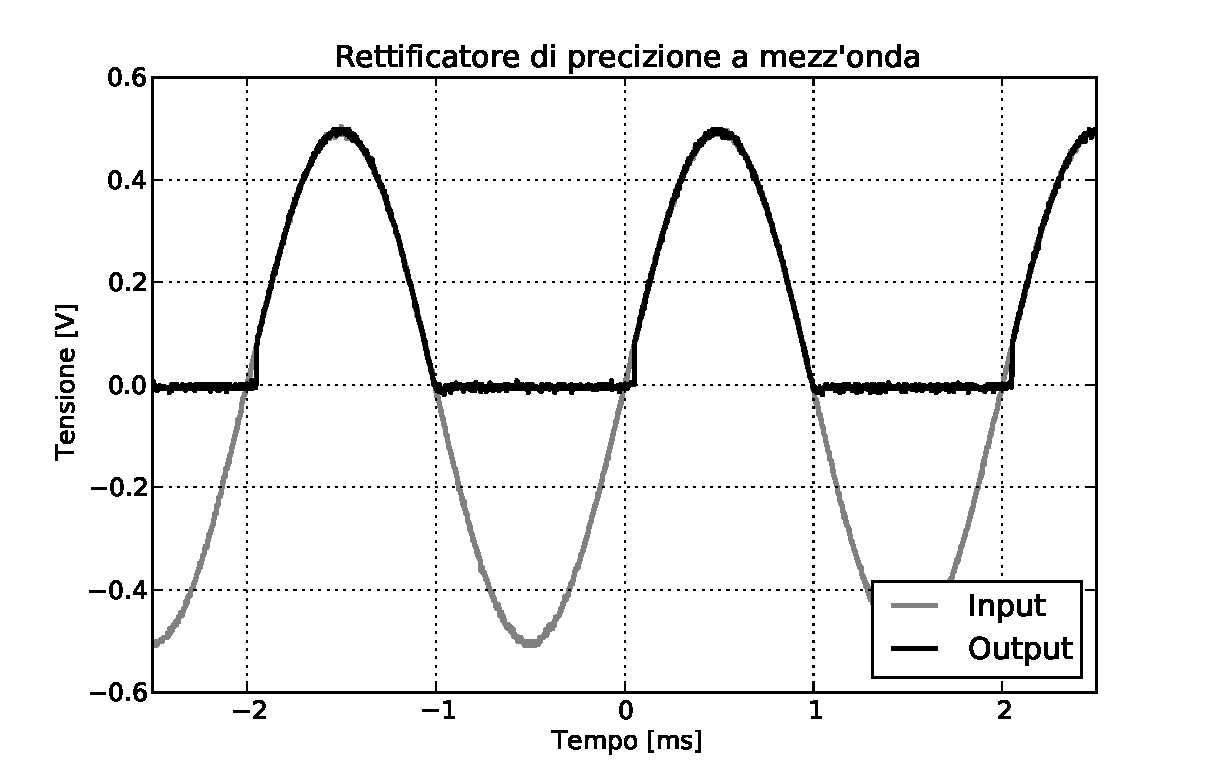
\includegraphics[width=0.7\textwidth]{figure/rett.pdf}
%        \caption{Questo grafico illustra l'andamento di $V\ped{out}$, linea nera, in funzione di $V\ped{in}$, linea grigia. Si nota chiaramente, come da previsioni, che la parte negativa del segnale in ingresso impediscse al diodo di condurre, pertanto la tensione di output risulta nulla. Inoltre, come si può osservare, il fronte di salita di $V\ped{out}$ presenta un leggero ritardo rispetto al segnale in ingresso $V\ped{in}$. Questo ritardo è stato stimato essere approssimativamente di circa $(152\pm10)\SI{}{\micro\second}$.}
%        \label{fig:radd_plot1}
%\end{SCfigure}
